\chapter{Návrh systému pro infračervený přenos dat}
\zkratka{LG} je založeno na optickém přenosu dat ze zbraně do vesty. Tato data jsou naprosto klíčová, nesou v sobě informace o tom, kdo je vyslal a chyba při přenosu nebo interpretaci těchto dat by mohla být fatální na stav hry. V krajním případě by mohla způsobit přičtení bodů špatnému hráči, což by při kumulaci způsobilo naprostou degradaci hry. Proto je potřeba se problematikou optického přenosu dat zabývat pečlivě.

Při \zkratka{LG} jsou data přenášena v infračerveném pásmu elektromagnetických vln, což odpovídá vlnovým délkám $\lambda \in \langle 760~\jedn{nm};~1~\jedn{mm}\rangle$. Tyto vlnové délky jsou pro lidské oko nedetekovatelné, což je podstatné k zachování smyslu a atmosféry hry.

\section{Požadavky na systém}
Systém musí být schopen vyslat po stisknutí spouště informace o tom, kdo vystřelil. Tuto informaci musí být také schopen přijmout, dekódovat a rozhodnout, jestli jsou data v pořádku, či přišla poškozená. Data by měla být schopna adresovat minimálně 12 hráčů a čas od výstřelu do vyhodnocení dat by měl být minimalizován (např. kvůli možné pokračující hře virtuálně mrtvého hráče.).

\section{Návrh přenášeného rámce}
Bylo rozhodnuto použít osm bitů pro adresu a šestnáct bitů pro kontrolní součet. Takto vytvořený adresovací prostor pokryje všechny hráče s dostatečnou rezervou pro možné rozšíření systému o interaktivní překážky. Hráči budou adresováni od nuly do $n$, kde $n = počet _{hráčů} - 1$.

\begin{figure}[H]
    \begin{center}
        \includegraphics[width=\textwidth]{img/ir-packet}
    \end{center}
    \caption{Obrázek struktury rámce}
\end{figure}

\section{Výběr IR vysílače}
IR vysílač má za úkol v relativně širokém rozsahu vzdáleností (přibližně 1 až 15 metrů, což odpovídá vzdálenostem, na které jsou od sebe hráči v laser game arénách vzdáleni) osvítit zásahové čidlo a předat mu informaci o tom, kdo jej zasáhl.

Z dostupných součástek na trhu byl hledán kompromis mezi cenou, výkonem a vyzařovacím úhlem.

IR lasery se při laser game příliš často nepoužívají, protože jejich paprsek je velmi úzký a nevytvořil by se kužel o dostatečném průměru, který by zasáhl hráče. Laser by se musel doplnit dodatečnou optikou, což by vyžadovalo další náklady. Proto se pro přenos dat využívají IR LED. U těchto diod je třeba vyřešit problém zcela opačný - výběr LED s dostatečně malým vyzařovacím úhlem.

Při experimentech s IR LED s různými vyzařovacími úhly se mi pro tento účel jevily jako ideální diody s vyzařovacím úhlem $12^\circ$, vložené do $10$~\jedn{cm} trubičky. Diody s menším vyzařovacím úhlem byly problematické při kratších vzdálenostech, protože vyzařovaný kužel byl příliš malý.

Důležitým parametrem IR LED je vlnová délka vyzařovaného záření - volba závisí na použitém přijímači. Pokud by měly vysílač s přijímačem rozdílnou vlnovou délku, nastával by útlum přenášeného signálu. Vybrána byla nejrozšířenější vlnová délka $940~\jedn{nm}$.

\section{Výběr IR přijímače}
IR přijímač má za úkol detekovat IR záření vysílané vysílačem. Vzhledem k tomu, že přijímače jsou integrované přímo ve vestě, je důležitým kritériem jejich velikost. Integrované přijímače jsou pro tento účel ideální - mají v sobě integrovanou fotodiodu, vstupní transimpedančí zesilovač, pásmovou propust, demodulátor i zesilovač, který má nastavitelné zesílení a snaží se udržet amplitudu výstupního signálu stabilní. A navíc, většina těchto zesilovačů má výstup typu otevřený kolektor, takže lze snímače spojovat bez nutnosti použití dalších součástek.

Důležitým parametrem je snímací úhel, v případě snímačů by bylo ideální, kdyby snímaly záření dopadající i pod úhlem $90^\circ$ stejně citlivě jako záření dopadající na snímač přímo pod nulovým úhlem. Takové snímače ale nejsou dostupné - snímače, které jsou na trhu, mají nejčastěji přijímací úhel $45^\circ$, pro použití při laser game to je ale málo. Ve výsledku byl nalezen přijímač OSRB38C9BA s úhlem $90^\circ$ a vlnovou délkou $940~\jedn{nm}$.

\begin{figure}[H]
    \begin{center}
        \includegraphics[width=0.7\textwidth]{img/OSRB38C9BA-direction}
    \end{center}
    \caption{Směrová charakteristika OSRB38C9BA, převzato z katalogového listu výrobce}
\end{figure}

\begin{figure}[H]
    \begin{center}
        \includegraphics[width=0.7\textwidth]{img/funkce-ir-detektoru}
    \end{center}
    \caption{Ukázka funkce ideálního integrovaného detektoru}
\end{figure}

Tento přijímač očekává signál modulovaný na nosný signál $37,9~\jedn{kHz}$. Podstatnou vlastností přijímače je tolerance výstupního signálu $\pm 200~\jedn{\mikro s}$ na vstupní testovací puls o šířce $600~\jedn{\mikro s}$. S tím je třeba počítat při návrhu komunikačního protokolu.

\section{Přenos IR signálu}
IR signál je přenášen od vysílače vzduchem k přijímači. IR signál má vlastnost, že se dobře odráží od bílých stěn, to lze pozorovat například na dálkových ovladačích ke spotřební elektronice, které fungují na stejných principech, pokud ovladač namíříme na bílý strop, IR záření se od něj odrazí a dostane se až k detektoru spotřebiče. Proto jsou stěny v LG arénách tmavé, aby záření pohlcovaly.

Přenášený IR signál musí být modulovaný na nosnou vlnu. Pokud by nebyl modulovaný, stačilo by na detektor jen posvítit, například ze zářivky a detektor by toto záření interpretoval jako náš požadovaný signál, přestože by se jednalo o rušení. Bohužel, namodulování signálu na nosnou vlnu nezabrání veškerému rušení do systému proniknout, navíc existují i LED osvětlení, jejichž budiče pracují právě na frekvenci nosné frekvence systému vest, čímž osvětlení kompletně zahltí komunikační kanál rušením. Proto je důležité v aréně používat kvalitní světelné zdroje s měniči pracujícími na odlišných-vyšších frekvencích.

\section{První návrh systému IR přenosu dat}
\begin{figure}[H]
    \begin{center}
        \includegraphics[width=\textwidth]{img/fake}
    \end{center}
    \caption{Zjednodušené schéma první verze systému pro IR přenos dat}
\end{figure}

\subsection{Vysílač}
Vysílač je založen na modulování \zkratka{UART} na \zkratka{PWM}, které generuje mikrokontrolér. Frekvence PWM je nakonfigurována na hodnotu $37,9~\jedn{kHz}$, protože na ni má IR detektor největší zisk. Změna střídy nastavuje dosvit vysílače.

Protože UART má klidový stav v logické stavu 1, je invertován pomocí hradla negace a s pomocí hradla AND namodulován na PWM. Kdyby nebyl invertován, vysílací LED by většinu času strávila vysíláním, což by zbytečně zvýšilo spotřebu a navíc by mohlo dojít k zahlcení detektoru.

\subsection{Přijímač}
Přijímač k dekódování přijatého signálu využívá UART integrovaný v mikrokontroléru. Klidový stav detektoru je díky integrovanému pull-up odporu v logické jedničce, pokud detekuje signál, je výstup stáhnut do logické nuly. Tohle chování detektoru je pro systém vhodné, protože vysíláme pouze nulové bity. Detektor je opatřen RC článkem, aby do něj nevnikalo rušení z napájecího vedení.

UART byl nastaven na přenosovou rychlost $2400~\jedn{bps}$. Na jeden bit trvá přibližně $416~\jedn{\mikro s}$. Perioda jednoho PWM pulzu je $23~\jedn{\mikro s}$, tedy na jeden bit připadá $16$ PWM pulzů. Vzhledem k toleranci detektoru je patrná příčina vznikání chyb při zahlcení, zkrátka přenosová rychlost je na použitý detektor příliš vysoká. Experimentálně byla vyzkoušena i nejnižší standardní přenosovou rychlost $1200~\jedn{bps}$ - jeden bit tedy trval $832~\jedn{\mikro s}$. Ale stále při posílání dat s velkým počtem nul docházelo velmi často k chybám - bylo možné ještě snižovat přenosovou rychlost, ale zahlcování detektoru by tím nebylo sníženo - proto bylo rozhodnuto o navrhnoutí vlatního komunikačního protokolu.

\subsection{Zhodnocení systému}
Tato koncepce přenosu není příliš spolehlivá. Pokud se vysílají data, která obsahují velké množství nul, po několika paketech dojde k zahlcení detektoru. To se projevuje tak, že se projeví tolerance detektoru $\pm200~\jedn{\mikro s}$, která deformuje přijímaný signál. UART tyto data poté dekóduje s velkou chybovostí. Díky CRC kontrole se sice vyhodnotí, že data jsou chybná, tudíž nedojde k usmrcení zasaženého hráče a přičtení bodů špatnému hráči, ale pokud hráč protihráče zasáhl a on přesto žije, degraduje to hru. Pokud se přeruší část packetu (poslední byte) při přenosu, UART tuto chybu neodhalí a od přerušení spojení nabude zbytek bitů hodnotu jedna.

\section{Druhý návrh systému IR přenosu dat}

\begin{figure}[H]
    \begin{center}
        \includegraphics[width=\textwidth]{img/ir-system}
    \end{center}
    \caption{Zjednodušené schéma druhé verze systému pro IR přenos dat}
\end{figure}

Tento systém vznikl jako náhrada systému předchozího. Je navržen tak, aby odolával problémům se shluky nul a korektně dekódoval data i při jejich deformaci o $\pm200~\jedn{\mikro s}$.

Systém už není založen na modulování protokolu UART na PWM signál. Byl inspirován komunikačními protokoly dálkových ovladačů, které jsou robustní a spolehlivé. Pro přenos byl navrhnut vlastní komunikační protokol - jak logická jednička, tak nula jsou reprezentovány pulzem a charakteristickou mezerou, takže pokud dojde ke ztrátě části packetu, problém je odhalen, protože dojde k porušení podmínek komunikačního protokolu.

\subsection{Komunikační protokol}
Komunikace začíná odesláním startovacího impulzu, poté následuje startovací mezera. Po této sekvenci následuje 24 period začínajících vždy datovým pulsem, který má pevnou délku, následovaným mezerou, která definuje zda-li se přenáší logická jednička či nula. Po dokončení posílání datových bitů následuje ukončovací pulz. Jednotlivé packety jsou od sebe navíc odděleny mezerou, která má definovanou minimální délku. Při vyhodnocování se počítá s tolerancí $\pm250~\jedn{\mikro s}$, což s rezervou pokryje toleranci optického přijímače.

\begin{table}[H]
  \caption{Definice časování komunikačního protokolu}
  \begin{center}
  	\small
	  \begin{tabular}{|l|r|}
	    \hline
	    \textbf{název} & \textbf{čas [\jedn{\mikro s}]} \\\hline\hline
	    \texttt{IR\_TIM\_START\_PULS}       &  5000     \\\hline
	    \texttt{IR\_TIM\_START\_SPACE}      &  5000     \\\hline
	    \texttt{IR\_TIM\_DATA\_PULS}        &   600     \\\hline
	    \texttt{IR\_TIM\_DATA0\_SPACE}      &   600     \\\hline
        \texttt{IR\_TIM\_DATA1\_SPACE}      &  1200     \\\hline
        \texttt{IR\_TIM\_END\_PULS}         &  3000     \\\hline
        \texttt{IR\_TIM\_PACKET\_SPACE}     & 30000     \\\hline
        \texttt{IR\_TIM\_TOLERANCE}         &   250     \\\hline
	  \end{tabular}
  \end{center}
\end{table}

\begin{figure}[H]
    \begin{center}
        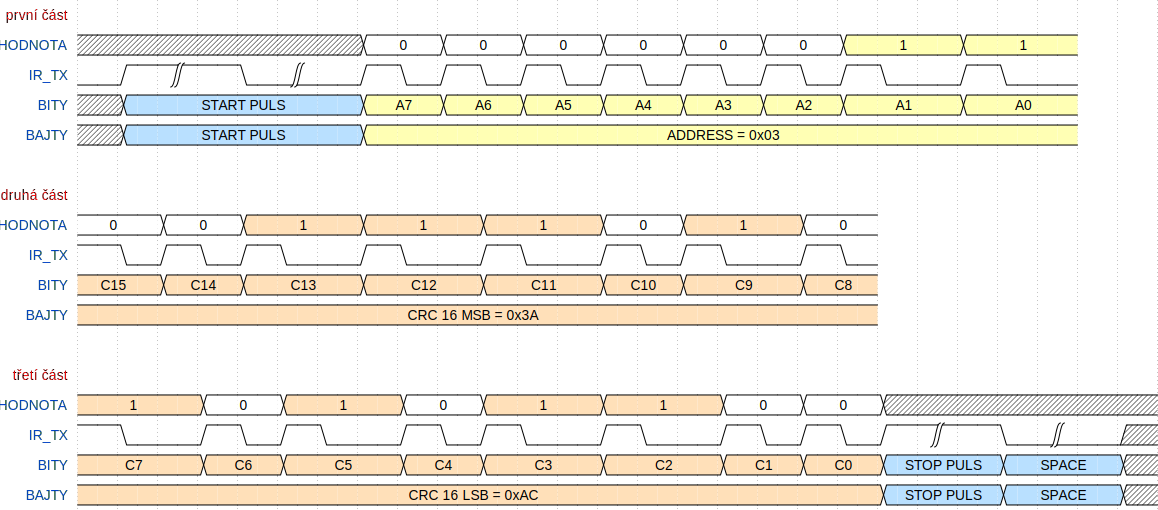
\includegraphics[width=\textwidth]{img/ir-protocol}
    \end{center}
    \caption{Ukázka jednoho rámce přenášeného IR protokolem}
\end{figure}

\subsection{Zhodnocení}
Tento protokol je spolehlivý, povedlo se jím opravit všechny nedostatky, kterými trpěla první navržená verze. Navíc došlo ke zjednodušení HW. V přijímači už není potřeba mít hradlo negace - z HW by se mohlo vypustit i hradlo AND a nahradit jej hradlem NAND, které je součástí IRTIM (IR timeru, který vznikne spojením timeru 16 a 17) integrovaným přímo v některých MCU řady STM32F0. Pro vysílač ale byl vybrán MCU, který integrovaným NAND hradlem nedisponuje.

Maximální doba přenosu jednoho rámce (plného logických jedniček), trvá $86,2~\jedn{ms}$. Minimální doba přenosu rámce (plného nul) je $71,8~\jedn{ms}$, maximální přenosová rychlost je $334~\jedn{bps}$ a minimální přenosová rychlost je $278~\jedn{bps}$. Dosažené přenosové rychlosti jsou sice mnohem nižší než v předchozí verzi, ale vzhledem k přenesenému objemu dat $24~\jedn{b}$ po stisku spoušti, je doba přenosu přijatelná.

Případné navýšení datové propustnosti protokolu by bylo možné pomocí snížení mezery mezi rámci.

%\begin{figure}[H]
    %\begin{center}
    %    \includegraphics[height=0.97\textheight]{img/model-ir-komunikace}
    %\end{center}
    %\caption{simulace časových průběhů komunikačního protokolu při přenosu nulového packetu}
%\end{figure}
